% Figure M9-Zheng-FACS hero: FACET on bead-purified Zheng17 FACS-sorted PBMC
% subpopulations with NATIVE cell-type labels. Generated by
% experiments/m9_zheng_facs.py --hero.
\begin{figure}[t]
 \centering
 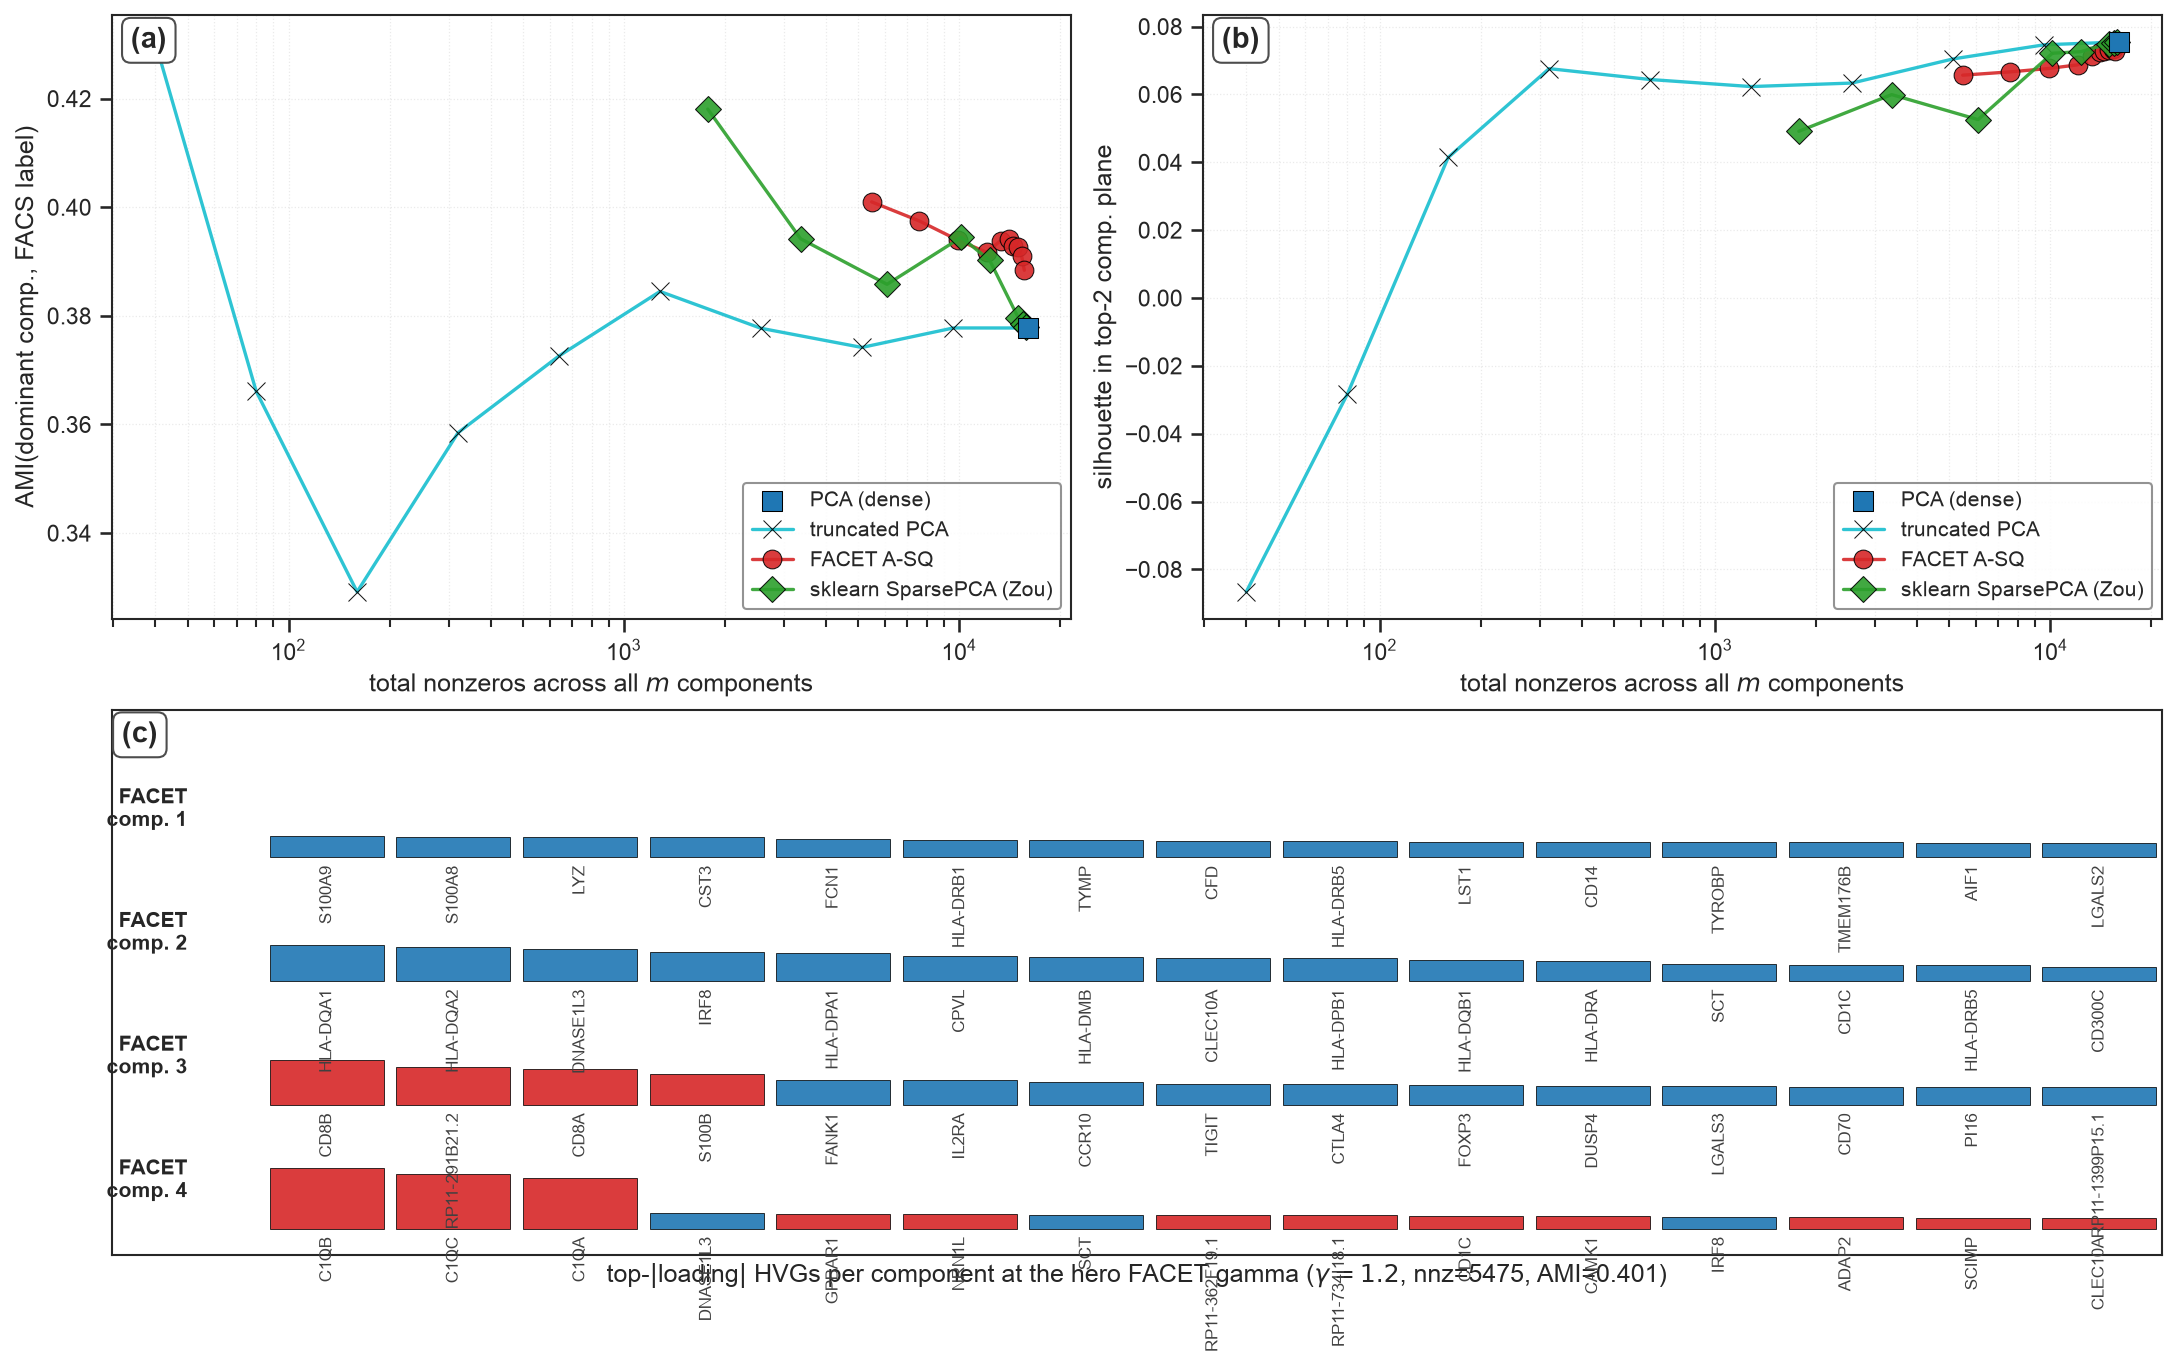
\includegraphics[width=\linewidth]{../shared/figures/generated/m9_zheng_facs_hero.png}
 \caption{\textbf{M9 Zheng17 FACS-sorted PBMCs, native cell-type labels.} Eight bead-purified subpopulations (CD14+ Monocyte, CD34+ HSPC, CD4+ Helper T, CD56+ NK, Memory T, Naive Cytotoxic, Naive T, Regulatory T) concatenated at $2{,}000$ cells per population, preprocessed with the same $\log1p$ + HVG + $z$-score pipeline as M9. Labels are the FACS gates, independent of any clustering step. \textbf{(a)}~AMI vs total nonzeros across all $m{=}8$ loadings. FACET A-SQ attains AMI $0.401$, above the dense-PCA ceiling at $0.378$, flipping the ranking seen on PCA-derived pseudo-labels in Fig.~\ref{fig:m9-scrna-hero}. \textbf{(b)}~Silhouette in the top-two component plane. \textbf{(c)}~Top-15 gene loadings per component at the hero FACET gamma.}
 \label{fig:m9-zheng-facs-hero}
\end{figure}
